\section{Description of Work Performed}
We defined several tasks in our proposal, and each of these tasks relates to topics learned in class. This section discusses the work performed for the project categorized by the relevant class topic.
\subsection{Waterfall Development Pattern}
One important objective for this project was to employ good software development practices, which meant including all stages of development and employing a development pattern. Using the waterfall development pattern, we first developed high-level ideas about our project, such as defining the problem our library would solve, and ended with working on more concrete tasks, such as defining unit tests for our software. We developed high-level requirements, functional requirements, and class and state diagrams for this project. After the problem definition, requirements, and architecture were defined, Each programmer performed high-level design, low-level design, construction, and testing steps on the tasks they were assigned. 

This work related to the workflows lab, the software engineering lecture where we learned key steps in the software engineering process, including the importance of establishing requirements early and choosing the correct development workflow.
\subsection{GitHub Repository}
After the more abstract stages of the waterfall development pattern were completed, we began to delegate tasks using the issue feature on GitHub. Up to this point, we had already been using GitHub as repository and Git as a version control system for our various diagrams and documents. However, at this point it would also become a place to delegate and collaborate. At the start of the project, each member was assigned three tasks to complete. These tasks were turned into issues, and most issues were turned into branches where the library's development took place. Issues were assigned to people, given tags, and placed on a project for later tracking. We also used the GitHub project to construct a timeline of when certain issues should be completed, and reminders were given to teammates when their tasks were nearing their due date. 

Once each issue was defined, the person assigned to the issue was asked to review it and determine if any other clarification was needed. Apart from that, the assignee could begin to work on that library feature and would eventually merge it into the main branch. 

Finally, once tests started to be written for the library, we implemented continuous integration by running all tests on GitHub and requiring them to pass before a branch can be merged into the main branch.

This work related to the "tools of the trade" lecture and labs 6 and 7, where we learned the importance of version control for stability and collaboration and the usefulness of GitHub for hosting a repository and coordinating group work.
\subsection{Object-Oriented Design}
We employed the object-oriented paradigm for our library using C++. In total, eight classes were used in our library. However, the Structure, Body, Edge, and Node classes were the most relevant classes because they defined the main objects that were used in the simulation. The full list of classes that were used is provided in Table \ref{tab:classes} along with their main purpose.
\begin{table}[H]
\centering
\caption{Okin Library's Classes}
\label{tab:classes}
\def\arraystretch{1.05}
\makebox[\textwidth][c]{
\begin{tabular}{|c|p{100mm}|}
\hline
\textbf{Class}                   & \textbf{Purpose} \\ \hline
Structure & Aggregate all bodies,nodes, and edges and provide an interface to the user for simulation  \\ \hline
Body   & Aggregate nodes and edges and provide a basis for minimal rigidity  \\ \hline
Edges  & define a connection between nodes and all properties related to that connection (distance, etc.)  \\ \hline
Nodes   & Encode the geometry of a structure  \\ \hline
LinAlg   & Perform linear algebra routines needed in the Structure class  \\ \hline
JsonParser   & Acts intermediary between input/output files defined in JSON and the Structure class  \\ \hline
JsonNode   & Provides a basic unit of data in the JsonParser's hierarchical structure  \\ \hline
tVelocity   & Encode the various types of velocities that can be defined by the user so they can be used in the simulation  \\ \hline
\end{tabular}
}
\end{table}

This work related to the "Lifecycle and OOP" lecture where we learned about the different characteristics of objects in OOP, such as encapsulation and inheritance, and how different objects can be related. This work also relates to programming best practices learned in homework 3.
\subsection {Compilation and External Libraries}
This library used CMake to simplify compilation and incorporate mature linear algebra libraries. A description of how this was done is given as well as justification for why we chose to do it this way.
\subsubsection{CMake}
For this library, CMake was used to generate the makefiles and complete all the library linking. CMake was chosen because it is adaptable to various system configurations and makes compilation straightforward for all users. We were also able to specify what kind of compiling options we wanted, such as which libraries to link or which compiler to use. In addition, we also implemented conditional compiling for the external libraries, where if the \texttt{find\_package(...)} command does not automatically find libraries, the code will still compile but with limited linear algebra abilities. 

% Figure \ref{fig:compilation} shows the flow of information in the CMake and Make process. The main workspace contained all the source and header files, which was added to the CMake sub-directories in the CMakeList. From the project workspace, we executed \texttt{cmake -S. -B./build} which then created the build directories which had the same file structure as the main project workspace. This build directory is system-dependent, and is ignored by Git when code is pushed to the repository. From the build file we then went into each source directory and executed the \texttt{make} command which then created the exectutables.

This work relates to several themes in class where we learned about pre-processing, compiling, linking, and installing. Linking external libraries into our library was similar to the PETSc lab, where we had to make sure we were using CMake correctly by ensuring it was able to find all the libraries required. The conditional compiling we used was similar to the examples shown during the ``Elements of Development" lecture. Setting up CMake in our file structure showed our mastery of the learning objectives presented in the ``Tools of the Trade" lecture.
% \begin{figure}[H]
% \centering
% 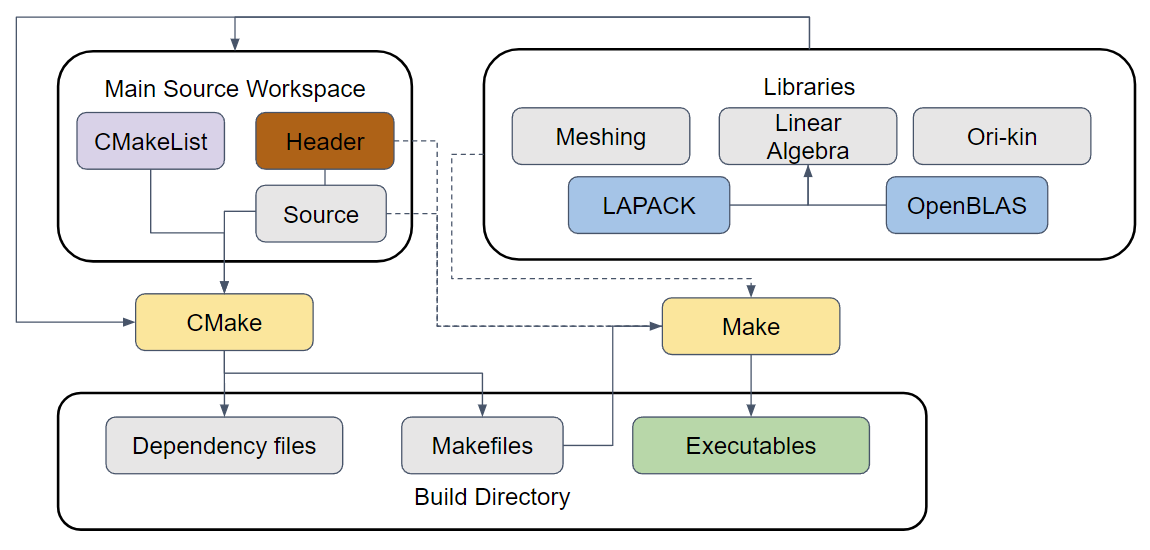
\includegraphics[width=0.8\textwidth]{Graphics/cmake.PNG}
% \caption{CMake compiling flow chart for the ori-kin library}
% \label{fig:compilation}
% \end{figure}
\subsubsection{Linear Algebra Libraries}
Linear algebra was required to determine the kinematically admissible motions of the origami pattern. The required linear algebra functions were described in the introduction. The two main functionalities required were the matrix-matrix multiplication and the pseudo inverse. The pseudo inverse was found using singular value decomposition (SVD),
\begin{equation} \label{eq:svd}
    C=U\Sigma V^T \longrightarrow C^+=U\Sigma ^{-1} V,
\end{equation}
where $C$ was almost always a non-square matrix. From Equation \ref{eq:svd}, it is clear that matrix-matrix multiplication is also required for this step as well as matrix inversion and transposition. While this and the matrix-matrix multiplication can be manually programmed, we decided to use a mature and performant external linear-algebra library. 

This work relates to course topics related to performance and linear algebra routines and libraries. Knowing it would be very difficult to create our own implementation of these algorithms that perform as well as these libraries on all platforms, using open-source linear algebra libraries allowed for efficient computing with minimal cache misses. Any linear algebra routines we implemented would have not used the underlying CPU architecture efficiently and would have resulted in high-bandwidth consuming operation.
\subsection{Visualization}
To provide a way to visualize simulations once they were complete, we extended the JSON parser input class to be able to write results out to a JSON file. Once written to a file, the simulation data could then be read by Python to create visualizations. To do this, we used the Blender visualization software along with the Blender Python module ``bpy". We wrote a Python script to load in all geometry data and combine it with the location history data to make the animations. Specifically, Blender requires an input Object and Mesh to define the visualization. The Object is analogous to a Structure in our C++ library while a Mesh contains all the geometric data, such as vertices, edges, and faces. However, generating a visualization from these two inputs alone generated a single static object. To enable us to view the actual folding motion, each data entry in the JSON file was written to a specific key frame. These key frames could then be played in succession to view the folding motion. From here the animations could be exported to many different video file formats.

This work relates to the scripting module, where we used the bash scripting language to perform similar data manipulation.
\subsection{Testing}
Unit and verification tests were written for our library, where unit tests would verify small components and verification tests would validate that our computations match the background mathematical model. Unit tests were written to verify the instantiation of the Node, Edge, Body, and Structure objects, paying special attention to how many objects were being copied versus passed by reference. Other unit tests verified that an object's properties in memory matched what was specified on the input file. Verification tests were written to verify computations performed in the intermediate stages of the initialization and simulation. For example, a test was written to verify that an angular target velocity specified in the input file was properly converted to a cartesian velocity. Most of these verification tests were constructed based on hand-calculated examples. These tests were incorporated with CMake so that they could be run automatically by us during development and by GitHub for continuous integration purposes.

This work relates to the "Lifecycle and OOP" lecture, the "Verification and Validation" lecture, and Homework 3 where we covered the different types of testing and used CMake to automatically run tests.


